\section{Discussion}\label{ch:disc}\raggedbottom
We only learned about few types of the many approaches undertaken by the participants. There are just too many strategies to examine every single one. Many good ideas, some of them maybe ground-breaking, are lost or even discarded by their designers because they receive a worse evaluation than common models.

After comparing the challenge performances of the previously presented methods in Sect. \ref{sec:comp}, this chapter reviews the challenges impact on Kaggle and CERN.

\subsection{Comparison of methods}\label{sec:comp}
Tab. \ref{tab:bestams} lists the best results we achieve, their hypothetical performance in the challenge is visualized by Fig. \ref{fig:ranks}. As stated in Sect. \ref{sec:lb}, we choose the best submissions by their public AMS, due to the hidden private leaderboard in the running challenge.

\begin{table}[h]
\begin{tabular}{|l|c|c|c|}
	\hline
	Classifier & public AMS & private AMS & private rank \\
	\hline
	Logistic Regression* & 2.04480 & 2.06934 & 1429 \\
	\hline
	k Nearest Neighbor* & 3.16941 & 3.18323 & 996 \\
	\hline
	sklearn.GradientBoostingClassifier & 3.44038 & 3.45097 & 838\\
	\hline
	XGBoost & 3.66421 & 3.71268 & 65 \\
	\hline
	XGBoost original submission & 3.72435 & 3.71885 & 45 \\
	\hline
	Winning submission (Neural Network) & 3.85059 & 3.80581 & 1 \\
	\hline
\end{tabular}

\vspace{1ex}

\emph{XGBoost original submission} and \emph{Winning submission} have been received from the official leaderboards and added as comparison, own approaches are marked with *. 
\caption{Best performances of used classification-methods}
\label{tab:bestams}
\end{table}

\begin{figure}[h]
	\centering
	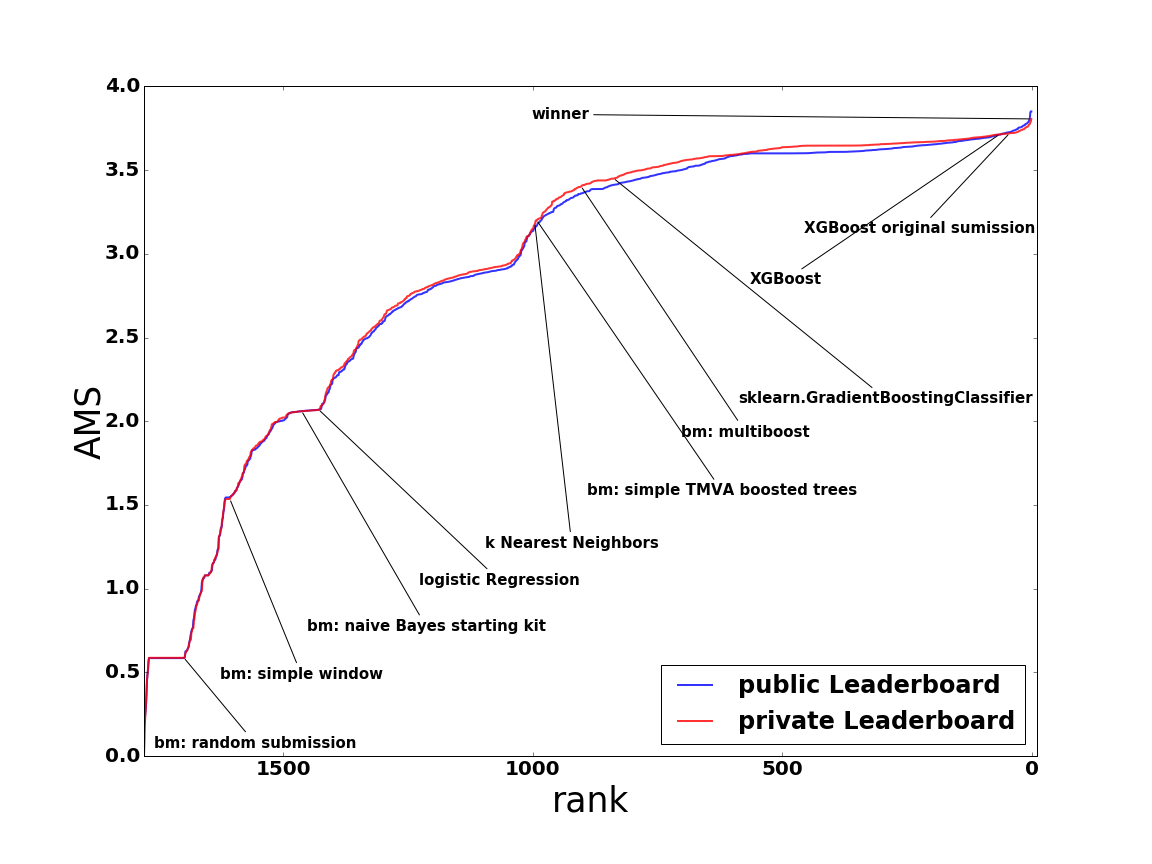
\includegraphics[width=\textwidth]{images/amscompare}
	\\Benchmarks placed by challenge-organizers have prefix bm.
	\caption{Public and private AMS plotted to equivalent rank}
	\label{fig:ranks}
\end{figure}

\subsubsection{Own approaches}
The first approach, Logistic Regression, only achieved poor AMS results. As opposed to other presented classifiers, this method responds best to Set 8. This is not that surprising as Set 8 was crafted, using an ensemble method. Its top submission is able to surpass the \emph{Naive Bayes starting kit} benchmark by only 0.00913 AMS. Both classifiers are considered as linear models, which can be an explanation for the resemblance of their AMS. As Naive Bayes is used as benchmark in the leaderboards, one can assume an AMS of about 2.1 is the top limit for linear classification. However, few competitors reported to the forums that they used linear models, in their cases Support Vector Machines. The best submission resulting in a public AMS of 2.7827 \cite{kaggleForum3}.

Being our other approach, k Nearest Neighbor(kNN) classification is able to outperform linear models significantly, scoring rank 996 on the private leaderboard. While this result is still within the lower half of ranked submissions, it is noteworthy close to the untuned TMVA benchmark with a difference of 0.01633 in private AMS, corresponding to five ranks on the private leaderboard. For the point of view that TMVA is an well-established tool in particle physics, the marginally worse performance of kNN is a small success.
As Fig. \ref{fig:setperf} visualizes, kNN is very sensitive to the choice of feature sets. Careful use of artificial features could give improvement to this classification and enable the model to surpass at least one more benchmark.
Over all, kNN was the only method we used that profited heavily from \emph{excluding} features of the data. This offers another possibility for improving it. An algorithm to weight features for this model on the basis of clustering could give information valuable for manual or automatic feature selection.

\begin{figure}[h]
	\centering
	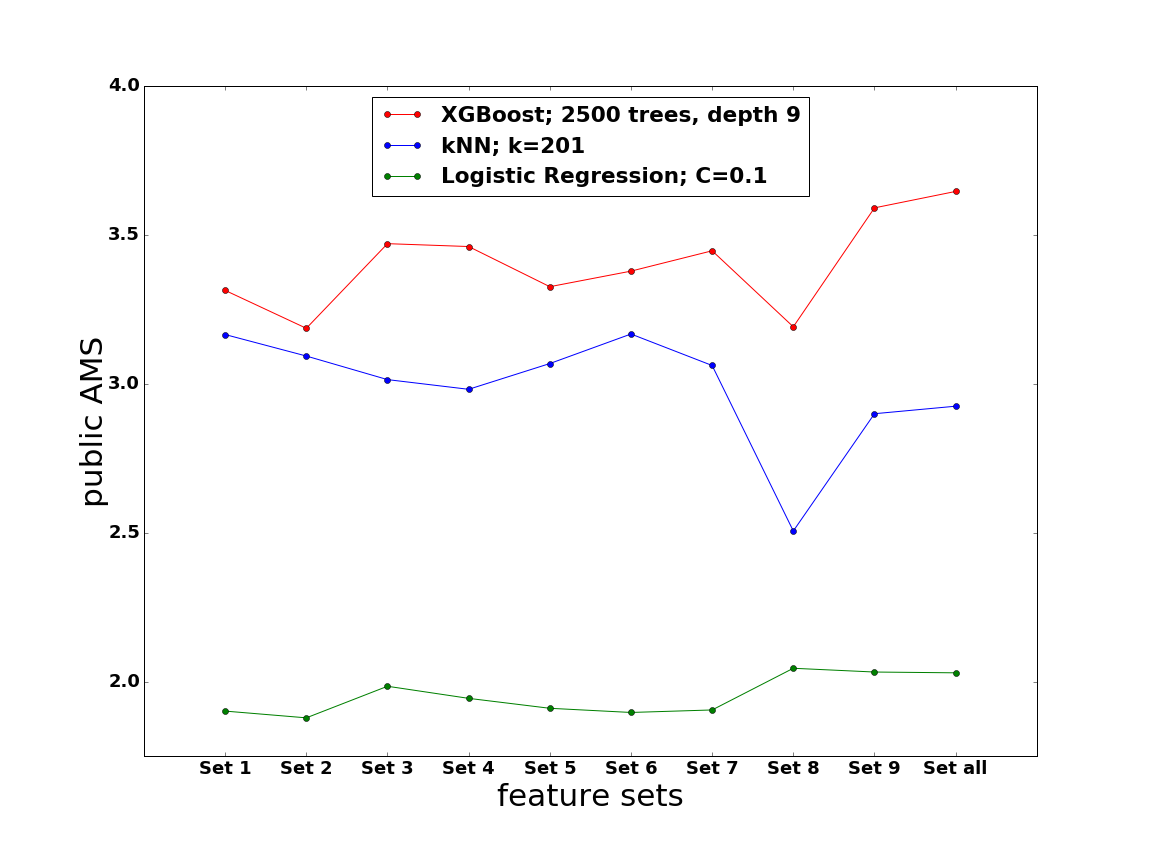
\includegraphics[width=\textwidth]{images/setperformance}
	\\Note the set sizes, listed in Tab. \ref{tab:feats}.
	\caption{Performances of classifiers for specific feature sets}
	\label{fig:setperf}
\end{figure}

\subsubsection{XGBoost and Neural Networks}
As mentioned, XGBoost gained quickly a fair amount of popularity after it has been presented in the Kaggle forums. We can understand this by comparing it to our own approaches.
Using low parameters, the package surpasses Logistic Regression with only 2 trees of depth 5 with \emph{eta}=0.1 in under 2.5 seconds in total (training and prediction time). For beating kNN, our personal best submission, XGBoost uses 40 trees with the same remaining parameters, having a total runtime of under 12.03 seconds.

Many submissions in the private top 500 used the package for their final submission. In Fig. \ref{fig:shakeup}, which appears in the next section, we can see a flat line around public rank 500. This is a group of submissions that all used XGBoost with same parameters and therefore experienced the same AMS difference with the transition to the private leaderboard \cite{hebert}.
Other participants were able to get a higher AMS with XGBoost. The differences in evaluation can be explained with different tuning efforts, we achieve a better score with heavy testing of different parameter settings. Our best XGBoost submission, measured by the public AMS, would be ranked on place 65.

The most common tuning for any classification method was proper feature engineering, though ,as previously stated, this procedure generally resulted in small improvements of AMS. However, even little improvement of classifiers could have resulted in a respectable amount of ranks, as concluded from Fig. \ref{fig:ranks}.

As we mentioned, an ensemble of Neural Networks delivered the winning submission, but it should be mentioned that the third place was also achieved by a method of this kind.
Since no testing of this type of classification has been undertook in this Thesis, we can not provide much insight to possibilities of improving this method. The winner of the challenge, Gábor Melis, reportedly used a number of artificial features \cite{meli14}. Courtiol Pierre (Rank 3) stated that increasing the size of his ensemble can improve the result slightly \cite{courtiol-3rd}.

\subsection{Impact of the Challenge}
While XGBoost did not win the Higgs Boson Machine Learning Challenge, it did have a strong impact on following Kaggle competitions. The most recently closed competition \emph{Prudential Life Insurance Assessment}\footnote{The competition closed on 15 February 2016.\\ URL: \url{https://www.kaggle.com/c/prudential-life-insurance-assessment}} features an ensemble of XGBoost classifiers as winning model, this and other methods involving XGBoost finished several competitions on Kaggle in top ranks \cite{xgbdoc}.

\subsubsection{Future Kaggle and CERN Collaborations}
After The Higgs Boson Machine Learning Challenge ended, many competitors criticized AMS evaluation by calculating the so-called \emph{Leaderboard Shake-up}. In the Kaggle Forums, this formula is often stated as \texttt{shake-up = mean[abs(private\_rank - public\_rank) / number\_of\_teams]}. We can express this mathematically as

\begin{equation}\label{eq:shakeup}
	\mathrm{Shake-up}:= s(v,b)= \frac{1}{N} \sum\limits_{i=1}^n \frac{|v_i-b_i|}{n}
\end{equation}

, where \begin{itemize}
	\item $v$ and $b$ are vectors of length $n$ containing private and public ranks, sorted w.r.t. affiliation to another, so $v_i$ and $b_i$ are the ranks of a single participating team.
	\item $n$ is the number of considered rank-pairs for the calculation for a specific subset of leaderboard-entries, like \emph{Top 10\% of private rank}.
	\item and $N$ is the total number of a challenges participating teams. $N$ = 1785 in case of the \emph{Higgs Boson Machine Learning Challenge}.
\end{itemize}

This is a measurement for differences in ranking between public and private leaderboard, it is common for the Kaggle community to rate a competition by this criterion, a low score being good. Given the final rankings, Eq. \eqref{eq:shakeup} calculates a total Shake-up of 0.033 and 0.050 for the Top 10\% participants. Summarized, competitors criticized the challenge mainly by two criteria. First, the amount of provided training data was too low. Community members argue that more test data used for the public AMS could prevent choosing overfitted submissions for the private leaderboard and subsequently improve the total Shake-up\cite{kaggleForum1,kaggleForum2}. Second, while AMS evaluation was used due to its relation to actual particle physics, it worked suboptimal for the challenge.

In CERNs following Machine Learning Challenge on Kaggle, \emph{Flavours of Physics: Finding $\tau \rightarrow \mu\mu\mu$}, these two criteria were addressed. More test data was provided to the challenge and the evaluation was calculated by \emph{weighted AUC}. Due to its favourable properties, AUC has been used by a number of top participants as objective function \cite{diaz14}. Fig. \ref{fig:shakeup} visualizes the Shake-up of this challenge and CERNs second Kaggle Challenge, latter having a total Shake-up of 0.038 and 0.013 for the Top 10\% participants. The smaller Shake-up within the top-ranks can be considered as improvement of the evaluation.
However, it has not been stated that these differences resulted directly from insights gained in the first competition.

\begin{figure}
	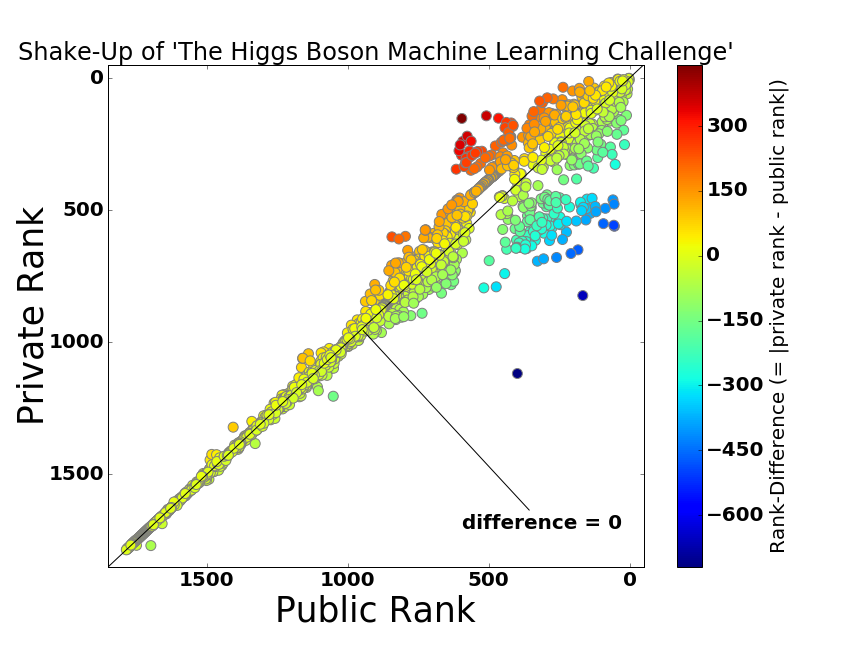
\includegraphics[width=.5\textwidth]{images/shakeup}
	\includegraphics[width=.5\textwidth]{images/flavshakeup}
	The leaderboard data was accessed from \cite{kaggle} with a simple python-script inspired by \cite{hebert}.
	\caption{Shake-up of \emph{The Higgs Boson Machine Learning Challenge} and \emph{Flavours of Physics}}
	\label{fig:shakeup}
\end{figure}

Though all the benchmarks provided by the challenge organizers have been surpassed by a considerable amount of submissions, the results ended up being controversial. An essential part of the challenge, optimizing the AMS, has been evaded by many competitors by using alternative objective functions. While this strategy opens up possibility for other research, many model designs that center AMS are probably dropped by their creators because they did not deliver significant improvements. 
The insight that CERN gained from the challenge taught more about winning on Kaggle than on designing new methods. All procedures that ended up in the top ranks are variations of established methods in data science, new, \emph{game changing} strategies were not discovered in the challenge. Further, the winning submission \emph{did not work at CERN}, due to compiling errors \cite{keglblog}.
However, a team was able to develop an original model based on theoretical results on AMS\cite{mack14}. The participants were invited to \emph{the Annual Conference on Neural Information Processing Systems 2014}(NIPS14) and presented their model. Their resulting submission was only ranked 461th.

\subsubsection{Data Analysis at CERN}
Overall the challenge still seemed to be a success for CERN, as they started and closed up an additional Kaggle challenge\footnote{The second challenge was called \emph{Flavours of Physics: Finding $\tau \rightarrow \mu\mu\mu$}.} in 2015. The first and second best submissions of this competition were generated using XGBoost. Though it has not been reported that the package is currently used for classification at CERN, it is still possible that it will be implemented in future upgrades performed on the LHC and its experiments. Meanwhile, the package experiences further gain in popularity, for instance it is used for a cloud service by Alibaba.\\
The creators recently received the \emph{John Chambers Award 2016} \cite{xgbgit}.

As the design of AMS was an effort to provide the competitors an objective function with physics background, the instability of AMS evaluation resulted in further research regarding usable objective functions for classification of LHC data\cite{HEPml}. On NIPS14, a \emph{new} AMS was presented, having more stable properties by including the variance of \emph{unknown background}. This could improve ATLAS own evaluation metric\cite{kegl14}.


%%%%%%%%%%%%%%%%%%%%%%%%%%%%%%%%%%%%%%%%%%%%%%%%%%%%%%%%%%%%%%%%%%%%%
% Leerseite bei zweiseitigem Druck
%%%%%%%%%%%%%%%%%%%%%%%%%%%%%%%%%%%%%%%%%%%%%%%%%%%%%%%%%%%%%%%%%%%%%
\ifthenelse{ \( \equal{\zweiseitig}{twoside} \and \not \isodd{\value{page}} \)}
	{\pagebreak \thispagestyle{empty} \cleardoublepage}{\clearpage}